%author: 	Patrik Goldschmidt
%title:		4. projekt
%subject: 	ITY
%faculty: 	FIT VUT Brno, Česká republika
%date:		04-08-2017

\documentclass[a4paper, 11pt]{article}

%%%%%%%%%%		Document settings & imports 		%%%%%%%%%%
\usepackage[T1]{fontenc}
\usepackage[utf8]{inputenc}
\usepackage{times}
\usepackage{indentfirst}
\usepackage{pdfpages}
\usepackage{graphics}
\usepackage{float}
\usepackage{geometry}
\geometry
{
	left = 2cm,
	top = 3cm,
	text = {17cm, 24cm}
}

%%%%%%%%		Custom commands and other settings 		%%%%%%%%

\usepackage[hidelinks, unicode]{hyperref}
	%Passing option hyphes to url package to allow hyphen url breaks
\PassOptionsToPackage{hyphens}{url}
	%Using package breakurl to allow breaks in url on Linux when not compiling in pdfLateX
	%Reference:	http://mirrors.nic.cz/tex-archive/macros/latex/contrib/breakurl/breakurl.pdf
\usepackage[hyphenbreaks]{breakurl}
\def\UrlBreaks{\do\/\do-}

\newcommand{\fakesubsection}[1]{%
  \par\refstepcounter{subsection}% Increase subsection counter
  \subsectionmark{#1}% Add subsection mark (header)
  \addcontentsline{toc}{subsection}{\protect\numberline{\thesubsection}#1}% Add subsection to ToC
  % Add more content here, if needed.
}

%%%%%%%%%%			Document information 		%%%%%%%%%%
\title
{	
	{\Huge Formal languages and compilers} \\[1em]
	{\huge Imperative language IFJ17 compiler implentation}
}
\author{\LARGE Team 006, variant II}
\date{\Large \today}

%%%%%%%%%%		Beginning of the document			%%%%%%%%%%
\begin{document}

%Title page
\makeatletter
\begin{titlepage}
	\pagenumbering{gobble}		% Turn off page numbering for this page
	
	\begin{center}
	{\Huge
		\textsc{Brno University of Technology}} \\[3.5mm]
	{\huge \textsc{Faculty of information technology}} \\

	\vspace{\stretch{0.9}}
	
	\@title \\[1.1em]
	\@author \\[1.2em]
	\@date
	
	\end{center}
	
	\vspace{\fill}

	\begin{minipage}[t]{0.77\textwidth}
	\vspace{\fill}
	\bigskip
	\medskip
	{\Large \textbf{Authors:}}	\\[1.2em]
	\begin{tabular}{| c| c | c | c |}
	\hline
	Leader 		& Name	 			& Login	 			& Points \\ \hline
				& Daniš Tomáš 		& \texttt{xdanis05} 	& $25 \%$		\\ \hline
	$\bullet$		& Goldschmidt Patrik	& \texttt{xgolds00}	& $25 \%$		\\ \hline
				& Hamran Peter		& \texttt{xhamra00}	& $25 \%$		\\ \hline
				& Pšenák Kamil		& \texttt{xpsena02}	& $25 \%$		\\ \hline
	\end{tabular}
	
	
	\end{minipage}
	\begin{minipage}[t]{0.28\textwidth}
	
	\hspace{4.55mm}	{\Large \textbf{Extensions:}}
	\begin{itemize}
		\item BASE
		\item CYCLES
		\item FUNEXP
		\item GLOBAL
		\item IFTHEN
		\item SCOPE
	\end{itemize}
	\end{minipage}
\end{titlepage}

%Page 2 - Document contents
\makeatother
\newpage
{\large \tableofcontents}

% Section: Introduction
\newpage
\pagenumbering{arabic}		% Turn of page numbering for this page
\setcounter{page}{1}

\section{Introduction}
The task to implement IFJ17 compiler was given as a semestral project for courses IFJ and IAL. Group of old friends back from the high school has decided to accomplish it together and that is how the team 006 was created. After doing an initial problem decomposition, labor was divided as follows:
\begin{itemize}
	\item \textbf{Tomáš Daniš} - Syntactic analysis, semantics checks, expressions evaluation, optimizations, tests definition
	\item \textbf{Patrik Goldschmidt} - Abstract data types and algorithms, documentation, lexical analyzer co-author, IFJ17 in-built functions, Makefile, script for regression tests
	\item \textbf{Peter Hamran} - Code generation, optimizations
	\item \textbf{Kamil Pšenák} - Lexical analysis, tests definition
\end{itemize}

This document further describes compiler development process and implementation details. Lexical analyzer FSA scheme as well as LL-grammar and LL-table are also included in the appendix section. 

% Sections: Interface & components
\section{Components and interface}

\subsection{IFJ17 API file}

For the special needs and mutually tied dependencies between various compiler components, we decided to create multi-purpose header file \texttt{ifj17\_api.h}. This file contains common data structures like \emph{token\_t} or \emph{symbol\_t}, which are used among most of the source files. For the sake of the best clarity and code readability, API file is included by all major components which is usually the only needed dependency for data structures used in our implementation.

\subsection{Lexical analyzer}

Lexical analyzer (\emph{scanner.c}) is implemented as a standard deterministic finite state automaton using \emph{C} \texttt{switch} command. Lexical analysis is done on per-call basis, where syntactic analyzer repeats requests for a new token during the compilation process. To serve parser's call, scanner module reads a couple of characters until it reaches character that does not belong to the actual token. At this point, extra character read is saved to the internal scanner buffer. Buffer is then used during the next token request - its value serves as a beginning of new a token. Buffer is then set to the empty state and token forming continues by reading the input file.

Communication between scanner and parser modules is based on passing tokens represented by \emph{token\_t} structure. Token structure is composed of an identifier, token attribute and special expression attributes. Based on the read character sequence, scanner fills identification field appropriately and sets particular attribute if the token is a literal.

Lexical analyzer also provides error detection using states \emph{error} and \emph{str\_error}. When an invalid character sequence is read, FSA switches to one of these error states. Reading states continues until white-space character or quotation mark in \emph{str\_error} state is read. Function then returns a lexical error. For advanced error recovery, scanner also supports line counting and error token value reporting. When the error occurs, user gets informed about the line at which the error occurred and also about a invalid token.

\vskip 0.5cm
\noindent Scheme of lexical analyzer is shown in the figure 1 on page \pageref{fig:scanner_scheme}.

\subsection{Syntactic analyzer}

The core of the compiler is syntactic analyzer (\emph{parser.c}). This module receives sequence of tokens from the scanner and validates if this sequence is a subset of the compiled language. If so, it also checks if the given construct is semantically correct and invokes generation of the output code. The module also analyses the semantics of the code to a certain extent to check for a possible optimizations.

The syntactic analysis was implemented with well-known recursive descent. This method was chosen because it was easier to implement, no extra stack was necessary and the resulting code structure is generally more readable. Expression analysis was implemented using PSA due to expression grammar. While it could be converted to an LL-grammar, we chose not to because of its simplicity and project requirements as well. LL-grammar and LL-table are included in the appendix section, pages \pageref{fig:ll_grammar} and \pageref{fig:ll_table} respectively.

However, our implementation deviates from the standards models in several ways:
\begin{itemize}
\item Placement of return statements is not checked using the LL-grammar but during the semantic analysis. This is done in order to simplify our LL-grammar.
\item We needed to find the way how to successfully link the execution of LL-analysis to the PSA algorithm and vice versa. This was accomplished by each of the two modules checking if the received token does not belong to the other module. If so, the other module was invoked with this token already pre-loaded. In the assignment without extensions, this could have been potentially problematic. However, we decided to implement FUNEXP extension, which provides more general functionality and eliminates this discrepancy. More information about this issue is provided in the extension section on page \pageref{sec:extensions}.
\item Way the \emph{end} expression is found. Algorithm for PSA analysis presented in the IFJ course supposes that the end of the expression is the end of the whole input. However, in a real-life scenario, this is not the case. Programs in the IFJ17 language still continue after an expression has ended. Therefore, we needed a way to detect when a received token is no longer a part of the expression. This was accomplished by constructing the follow set the \emph{<expr>} non-terminal. When one of the terminals from this set was received, we knew that it is no longer part of the expression and we artificially generated input of the PSA algorithm.
\item After the end of the program, there can be any number of EOL characters which are not detected using the grammar but are discarded until an other character is reached. If this character is not EOF, a syntactic error has occurred.
\end{itemize}

Semantics analysis is executed concurrently with the syntactic analysis. It has been implemented using a semantic stack for data passing between functions, symbol table and global state variables. Global state variables provide information about the context of the program such as block depth, name of the current function (if any) or which block of the code is currently being analyzed. The semantic stack collects data from multiple related functions, which are then retrieved in a single place where they are validated and used for code generation. A set of rules that define input and output for each function can be found in the appendix section on page \pageref{fig:sem_stack_rules}.

The symbol table is used for collecting information about functions and variables according to the standard implementation.

\subsection{Code generator}

Generator module creates output of the compilation process in the form of three address code IFJcode17. This code is then furtherly processed by interpreter \emph{ic17int}, which was provided with the assignment.

Like scanner, code generation is invoked by calls from the parser during the compilation process. Communication between these 2 modules can be split into several stages. Firstly, parser sets up instruction operands and internal logic, which then affects the generation process. Data is passed via a \emph{tstack} data structure, which was initially used for communication between the scanner and parser. Since generator needs almost all information contained in the token, we decided to re-use and slightly adjust this structure to facilitate parser and generator communication. After the stack is set, parser calls generator routine with a specific ID that represents particular instruction to be generated. Every instruction follows specific stack management rules - number of stack elements to be pushed, popped, swapped or edited. Code is firstly generated into the instruction list \texttt{ilist\_t}. This approach has several advantages, since the code can be optimized and is easily disposed if the compilation process fails. After optimization process is done, generator transforms instruction list contents into the instructions themselves. According to the assignment details, generated code gets printed to the standard output.

During the generation process, several issues need to be addressed. One of them is uniqueness of the generated variables and labels. Our solution solves this situation by using internal counters, whose value is preserved during the different invocations. Counter incrementation occurs after every expression evaluation, since temporary variable is created to store the result internally. Identifier of the generated variable is affected by parser, which specifies its name via value in the token structure. However, names for internal labels of loops, if statements and others are managed purely by the generator.

To achieve better generated program performance, compiler also provides few optimization techniques. Most of them are provided by parser, but generator handles some of them by itself. One of these optimizations is automatic in-built functions inlining. Using this method, in-built function bodies of \emph{Asc()}, \emph{Chr()}, \emph{Length()} and \emph{SubStr()} are straightly placed into the generated code. This effectively eliminates the cost of the jump instructions during the functions call.

\subsection{Algorithms and data structures}

\subsubsection{Symbol table}

According to the project requirements for variant II, symbol table is implemented using hash table. To achieve least hash collisions, acceptable performance and simplicity of implementation, Fowler-Noll-Vo (FNV) hash algorithm was chosen. Symbol table in this project uses FNV-1a variant with 32-bit flavor. This choice was inspired mainly by \cite{stackexch_sw_hash}. Specific implementation details and used magic numbers are based on one of the function author's blog \cite{noll_fnv}.

Symbol table itself is implemented as a local array of pointers to \emph{stab\_item\_t} structure. For the optimal performance/memory ratio, we decided to set a table size to 300 elements. Structure consist of the (\emph{symbol\_t}) data and pointer to the next item. Hash table items are thus mutually interconnected as a regular linked list. Key on which the hashing is based is the identifier contained in the symbol itself. Searching, inserting, deleting and other hash table operations are then based on the symbol ID contained in the hash table item.

Specialty of this hash table is that user is able to iterate though it using a \emph{stab\_iterator\_t} structure and in-built functions \emph{stab\_iterate\_set} and \emph{stab\_iterate\_next}. This functionality comes handy during semantics checks and output code optimization.

\subsubsection{PSA stack}

Stack for precedence syntactic analysis (\emph{tokenstack.c}) is composed of tokens with basic push, pop and top functionality. However, PSA algorithm requires specific stack functionality, so this stack was was needed to be adjusted accordingly. Returning topmost terminal is served via \emph{tstack\_get\_topterm()} function. Implementation also provides functionality to push desired token after the topmost terminal. To facilitate specific PSA requirements, stack also contains a sentinel value, which represents $\$$ in the PSA algorithm. This sentinel value is automatically added to the stack upon its initialization and can not be popped. Stack is then considered empty when it contains only a sentinel value.

Stack is also implemented fully dynamically. Dynamic size is achieved by internal implementation, which is basically a doubly-linked list. For reducing number of malloc calls, stack is pre-allocated upon initialization and when its maximum size reached, an expansion occurs. Using this approach, its size is theoretically limited only by the host's memory limitations.

\subsubsection{Instruction list}

Instruction list module \emph{ilist.c} provides an interface for storing instructions prior their optimization and generation. List is internally represented as a doubly-linked list, which also stores number of instructions currently in the list. This value is used for output code optimization and can be determined using \emph{ilist\_size()} function. Instruction list module further provides other regular doubly-linked list functions discussed during IAL course.

\subsubsection{Dynamic string}

Dynamically-sized string module \emph{str.c} provides C++ string pseudo-equivalent data structure. Module defines  \emph{string\_t} data structure, which is internally represented as a current length of the string, allocated size and C string type \emph{char *}. Dynamic string is pre-allocated to 128B and eventually reallocated to another +128B when its maximum size is reached. Manipulating the string is done via module functions, which support adding another char to the string, comparing between strings, conversion to the C-type strings and vice versa. This functionality is essential requirement for the scanner to build-up a token and pass it to the parser.

% Section: Development
\section{Development}

\subsection{Development cycle and project management}

Considering a fact that project requirements were known before the start of the development process and their change was not expected, choosing a waterfall development method would be more than appropriate. However, based on the unnecessary administrative overhead and lack of experience of project's programmers, we decided to stick with agile development techniques.

Development itself was preceded by a study phase and problem decomposition. Labor was divided based on the experience, skills and personal preferences. Since the development and study stages were partially overlapping, agile development has proven to be very effective. Inner requirements between different modules were often changed, so we needed to adapt to those changes and even occasionally rework modules to support desired functionality. 

To track our progress and discuss relevant issues, regular team meetings were held on weekly basis. For better cooperation, control version system \emph{git} was used. Many agile development techniques like pair programming, continuous testing and regular code reviewing were also applied.

\subsection{Testing and validation}

As expected, many errors during the development process arose. Some errors were revealed using unit tests, but most of them appeared when we connected the modules together. These were linked mainly to incompatible interface between modules due to different interpretation of the issues by authors of modules. Our custom tests helped us to find most of these bugs and fix them.

Discussing this topic, we would also like to thank Martin Kobelka's team for providing numerous number of tests and other tools used for IFJ project development. These definitely helped many teams including ours.

% Section: Conclusion
\section{Conclusion}

We definitely have to admit that this project was rather challenging, though it still taught us a lot not only about compilers and their design, but also about bigger team projects and how important internal team management and communication is. Some time still could be used for debugging and optimization purposes, but we definitely think that our final product is in the good shape and it should be able to correctly process source code IFJ17, detect various errors and create output 3-address code ready for further interpretation.

%Section: Citations
\newpage

\begin{thebibliography}{99}
	\bibitem{stackexch_sw_hash} BOLD Ian. Hash algorithms efficiency comparison. [online], April 2012. Available at: \texttt{\url{https://softwareengineering.stackexchange.com/questions/49550/which-hashing-algorithm-is-best-for-uniqueness-and-speed}}. Seen 3.12.2017.
	\bibitem{noll_fnv} NOLL Landon Curt. FNV Algorithm Overview. [online] June 2009, updated: March 2014. Available at: \texttt{\url{http://www.isthe.com/chongo/tech/comp/fnv/}}. Seen 3.12.2017.
\end{thebibliography}

%Section: Appendix: Extensions
\newpage
{\raggedright
	\section{Appendix}
}

\subsection{Extensions}
\label{sec:extensions} 

\subsubsection{BASE}

For the BASE extension purpose, support for extra tokens \texttt{\&b}, \texttt{\&h} and \texttt{\&o} needed to be added. After receiving this character sequence and at least one valid number belonging to the particular base, value gets converted to decimal using \texttt{strtol()} \emph{C} function. If no valid number in specified base is received, value of $0$ is implicitly returned. This process is done purely in the scanner module. Parser then receives decimal value in the token and is unaware that any conversion has happened.

\subsubsection{CYCLES}

CYCLE extension added support for \texttt{for} and \texttt{do...loop} cycle types. This also included support for loop flow control statements \texttt{exit} and \texttt{continue}. Implementation of this required us to track what cycles are we in at any point of the code analysis. This was accomplished using a semantic stack and a global variable counting cycle depth. \texttt{For} type cycles also required implementation of scope block variable validity tracking system. This eventually led us to the SCOPE extension implementation as well.

\subsubsection{FUNEXP}

FUNEXP extension required that functions are made as a part of expressions, which are normally analyzed with the PSA algorithm. However, argument list in the function call is not suitable to be analyzed by the PSA in a readable manner. Therefore, tighter cooperation between PSA and LL analysis was needed to be implemented. This is because argument list of functions is once again analyzed with LL analysis while the arguments themselves are expressions and are therefore analyzed with the PSA. In this manner, the two modules can call each other infinitely and we needed to ensure that correct data are passed between them.

The biggest problem was detecting whether during argument analysis, received right bracket is part of the expression or signifies the end of the function call. This was implemented by expanding the capabilities of our PSA table to be able to distinguish these two cases. In short, if an unmatched right bracket was found, the table reported the end of the function call. If this unmatched bracket was indeed an error, it was detected a few steps later during the LL-analysis.

\subsubsection{GLOBAL}

Extension GLOBAL required implementation of FREEBasic \texttt{global} and \texttt{static} variable types. To provide this functionality, variable shadowing was needed to be implemented. For this purpose, we used global symbol table shared for both variables and functions. Global symbol table combined with the global frame provided by IFJcode17 was sufficient for all the needs and this extension could be implemented.

\subsubsection{IFTHEN}

IFTHEN extension added support for standalone \texttt{If-then} and \texttt{elseif} statements. In this case, situation when the generator is unaware of number of labels and conditional jumps that have to be generated. This happens because we are unable to tell how many \emph{elseif} statements will follow. Problem was addressed by redirecting the code generation to the auxiliary instruction list.

IFTHEN rozšírenie pridáva podporu osamelých If-then statementov a elseif statementov.
V tomto prípade nastáva situácia kedy vopred nevieme ako je potrebné vygenerovať návestia
a podmienené skoky pre IFJcode17 z dôvodu potencionálne viacnásobného výskytu elseif statementov.
Tento problém sa odstránil pozastavením generácie kódu do inštrukčného listu 
a následným presmerovaním generácie tela podmieneného výrazu. Pri narazení na ďalšiu časť
podmieneného výrazu dokončíme generáciu predchádzajúce a vygenerované inštukcie sa pridajú
do hlavného inštrukčného listu.

listy, prelinkovanie v generatore z dovodov, ze nevieme, kolko else-if sa tu bude nachadzat
podmienena generacia lablov, rebranchovanie na tela

\subsubsection{SCOPE}

SCOPE extension required recursive block placement as well as correct visibility for shadowed variables in parent blocks. For this purpose, we implemented a variable depth stack (\texttt{vdstack.c}), which holds information about a single identifier and all its IFJcode17 possible names in various scope blocks. Each entry in this stack also contains information about scope block depth in which this name is used. At the end of the block, we iterated through the local symbol table and popped all the entries for the names that just went out of the scope.  This proved to be advantageous because all visibility handling was done during code analysis and no extra checks were necessary in the generated code.

% Section: Appendix: DFSA scheme
\newpage
\fakesubsection{Scanner scheme}

\begin{figure}[h]
	\centering
	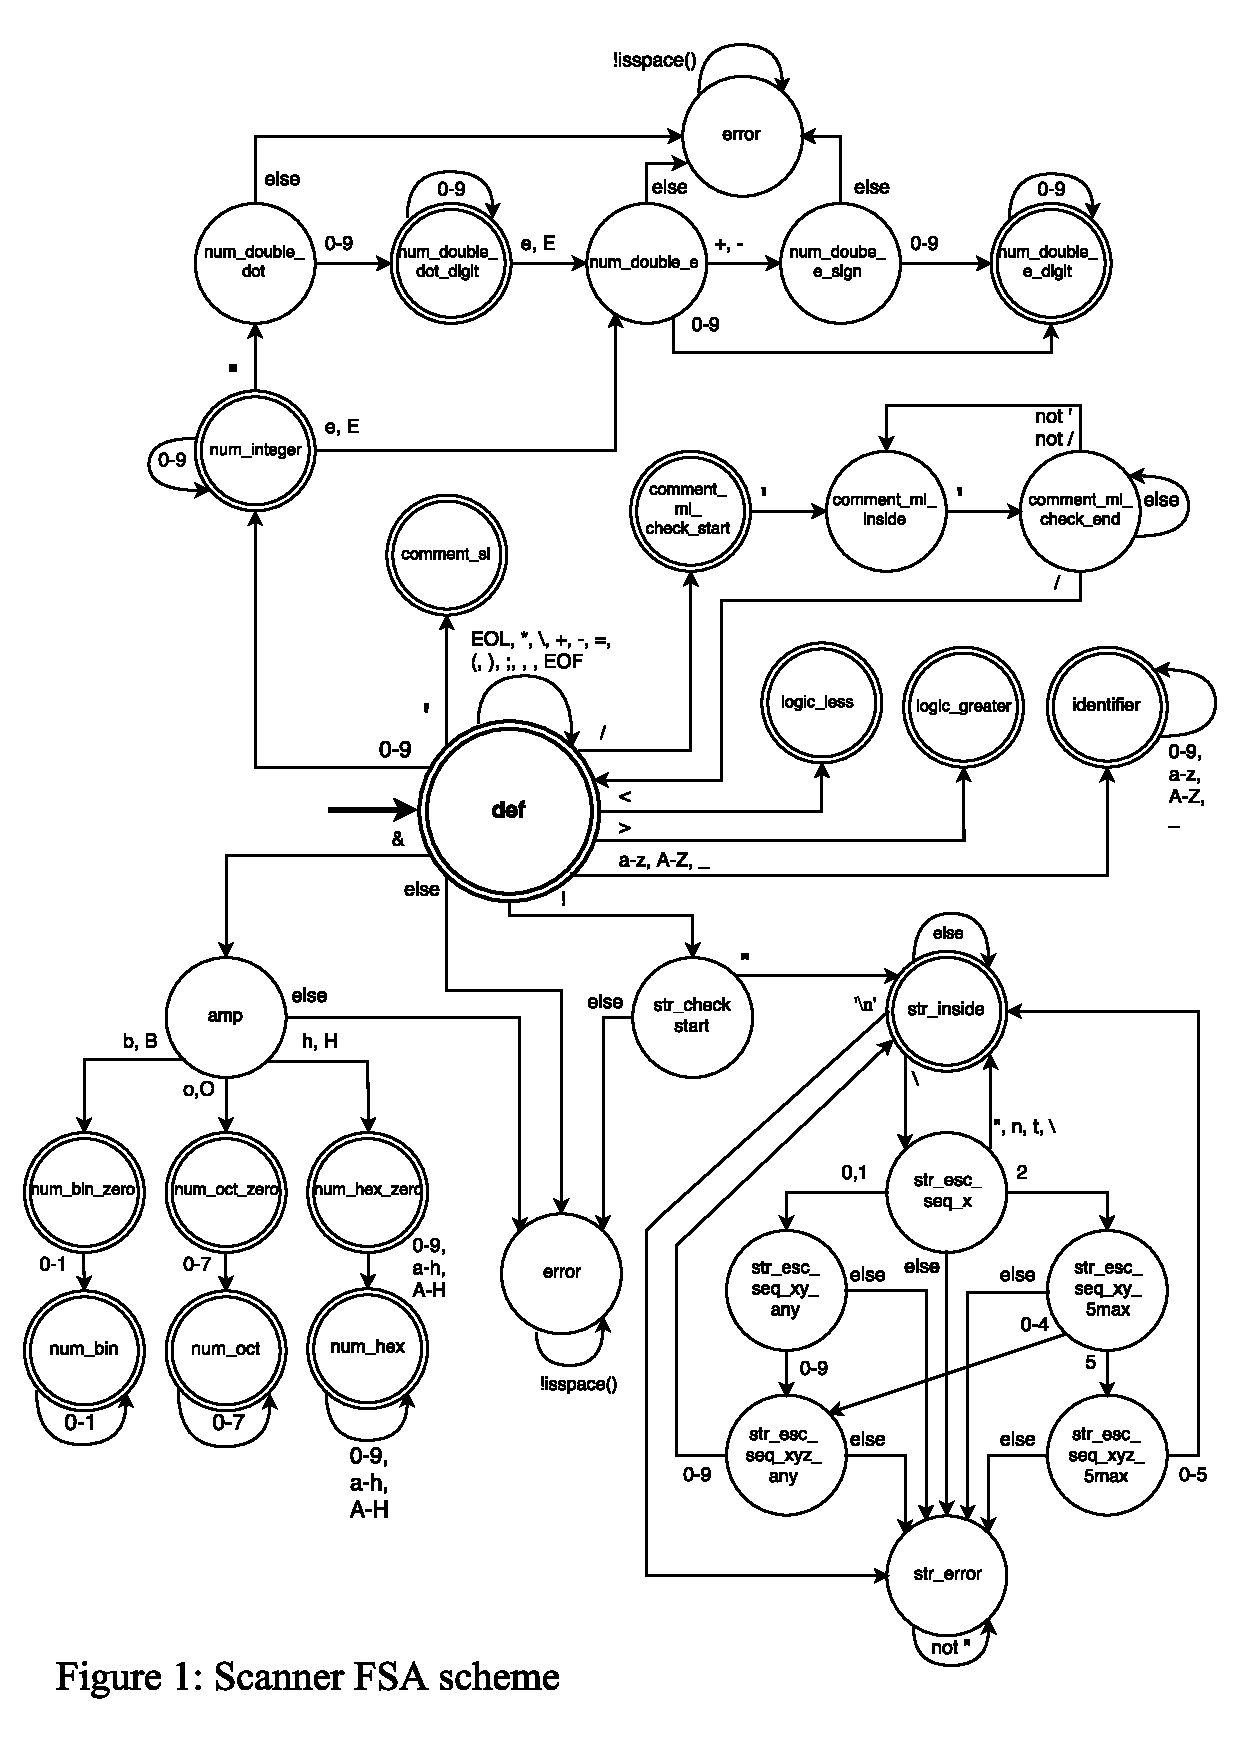
\includepdf[scale=0.87, pages={1}]{./attachments/scanner_scheme.pdf}
	\label{fig:scanner_scheme}
\end{figure}

% Section: Appendix: LL-grammar
\newpage
\label{fig:ll_grammar}
{\LARGE Figure 2: LL-grammar}
\fakesubsection{LL-grammar}
\bigskip

\begin{table}[H]
\begin{tabular}[l]{l l p{10cm}}
\textit{<prog>} & $\rightarrow$ & \textit{<decl\_list>} Scope EOL \textit{<stat\_list>} End Scope EOF \\
\textit{<decl\_list>} & $\rightarrow$ & \textit{<var\_decl>} \textit{<decl\_list>} \\
\textit{<decl\_list>} & $\rightarrow$ & \textit{<func\_decl>} \textit{<decl\_list>} \\
\textit{<decl\_list>} & $\rightarrow$ & \textit{<func\_def>} \textit{<decl\_list>} \\
\textit{<decl\_list>} & $\rightarrow$ & \textit{<empty\_statement>} \\
\textit{<decl\_list>} & $\rightarrow$ & $\varepsilon$ \\
\textit{<func\_decl>} & $\rightarrow$ & Declare Function id ( \emph{<param\_list>} ) As \emph{<type>} EOL \\
\textit{<func\_def>} & $\rightarrow$ & Function id ( \textit{<param\_list>} ) As \textit{<type>} EOL \textit{<stat\_list>} End Function EOL \\
\textit{<var\_decl>} & $\rightarrow$ & Dim \textit{<opt\_scope\_modifier>} id As \textit{<type>} \textit{<opt\_initialiser>} EOL \\
\textit{<var\_decl>} & $\rightarrow$ & Static id as \textit{<type>} \textit{<opt\_initialiser>} EOL \\
\textit{<param\_list>} & $\rightarrow$ & \textit{<param>} \textit{<param\_list\_cont>} \\
\textit{<param\_list>} & $\rightarrow$ & $\varepsilon$ \\
\textit{<param>} & $\rightarrow$ & id As \textit{<type>} \\
\textit{<param\_list\_cont>} & $\rightarrow$ & , \textit{<param>} \textit{<param\_list\_cont>} \\
\textit{<param\_list\_cont>} & $\rightarrow$ & $\varepsilon$ \\
\textit{<opt\_scope\_modifier>} & $\rightarrow$ & Shared \\
\textit{<opt\_scope\_modifier>} & $\rightarrow$ & $\varepsilon$ \\
\textit{<opt\_initialiser>} & $\rightarrow$ & = \textit{<expr>} \\
\textit{<opt\_initialiser>} & $\rightarrow$ & $\varepsilon$ \\
\textit{<type>} & $\rightarrow$ & Integer \\
\textit{<type>} & $\rightarrow$ & Double \\
\textit{<type>} & $\rightarrow$ & String \\
\textit{<stat\_list>} & $\rightarrow$ & \textit{<statement>} \textit{<stat\_list>} \\
\textit{<stat\_list>} & $\rightarrow$ & $\varepsilon$ \\
\textit{<statement>} & $\rightarrow$ & \textit{<assignment>} \\
\textit{<statement>} & $\rightarrow$ & \textit{<read\_statement>} \\
\textit{<statement>} & $\rightarrow$ & \textit{<print\_statement>} \\
\textit{<statement>} & $\rightarrow$ & \textit{<scope\_statement>} \\
\textit{<statement>} & $\rightarrow$ & \textit{<selection\_statement>} \\
\textit{<statement>} & $\rightarrow$ & \textit{<iteration\_statement>} \\
\textit{<statement>} & $\rightarrow$ & \textit{<return\_statement>} \\
\textit{<statement>} & $\rightarrow$ & \textit{<empty\_statement>} \\
\textit{<statement>} & $\rightarrow$ & \textit{<var\_decl>} \\
\textit{<statement>} & $\rightarrow$ & \textit{<iteration\_control\_statement>} \\
\textit{<assignment>} & $\rightarrow$ & id = \textit{<expr>} EOL \\
\textit{<read\_statement>} & $\rightarrow$ & Input id EOL \\
\textit{<print\_statement>} & $\rightarrow$ & print \textit{<expr>} ; \textit{<expr\_list>} EOL \\
\textit{<expr\_list>} & $\rightarrow$ & \textit{<expr>} ; \textit{<expr\_list>} \\
\textit{<expr\_list>} & $\rightarrow$ & $\varepsilon$ \\
\textit{<scope\_statement>} & $\rightarrow$ & Scope EOL \textit{<stat\_list>} End Scope EOL \\
\textit{<selection\_statement>} & $\rightarrow$ & If \textit{<expr>} then EOL \textit{<stat\_list>} \textit{<alternative\_statement>} End If EOL \\
\textit{<alternative\_statement>} & $\rightarrow$ & elseif \textit{<expr>} then EOL \textit{<stat\_list>}  \textit{<alternative\_statement>} \\
\end{tabular}
\end{table}

\begin{table}[H]
\begin{tabular}[l]{l l p{10cm}}
\textit{<alternative\_statement>} & $\rightarrow$ & else EOL \textit{<stat\_list>} \\
\textit{<alternative\_statement>} & $\rightarrow$ & $\varepsilon$ \\
\textit{<iteration\_statement>} & $\rightarrow$ & for id \textit{<opt\_type\_decl>} = \textit{<expr>} to \textit{<expr>} \textit{<opt\_step>} EOL \textit{<stat\_list>} Next \textit{<opt\_id>} EOL \\
\textit{<opt\_type\_decl>} & $\rightarrow$ & as \textit{<type>} \\
\textit{<opt\_type\_decl>} & $\rightarrow$ & $\varepsilon$ \\
\textit{<opt\_step>} & $\rightarrow$ & step \textit{<expr>} \\
\textit{<opt\_step>} & $\rightarrow$ & $\varepsilon$ \\ 
\textit{<opt\_id>} & $\rightarrow$ & id \\
\textit{<opt\_id>} & $\rightarrow$ & $\varepsilon$ \\
\textit{<iteration\_statement>} & $\rightarrow$ & do \textit{<do\_cycle>} EOL \\
\textit{<do\_cycle>} & $\rightarrow$ & EOL \textit{<stat\_list>} Loop \textit{<opt\_cond>} \\
\textit{<do\_cycle>} & $\rightarrow$ & \textit{<cond>} EOL \textit{<stat\_list>} Loop \\
\textit{<opt\_cond>} & $\rightarrow$ & \textit{<cond>} \\
\textit{<opt\_cond>} & $\rightarrow$ & $\varepsilon$ \\
\textit{<cond>} & $\rightarrow$ & \textit{<do\_mode>} \textit{<expr>} \\
\textit{<do\_mode>} & $\rightarrow$ & until \\
\textit{<do\_mode>} & $\rightarrow$ & while \\
\textit{<return\_statement>} & $\rightarrow$ & return \textit{<expr>} EOL \\
\textit{<iteration\_control\_statement>} & $\rightarrow$ & \textit{<control\_statement>} \textit{<cycle\_type>} \textit{<cycle\_type\_list>} EOL \\
\textit{<control\_statement>} & $\rightarrow$ & Exit \\
\textit{<control\_statement>} & $\rightarrow$ & Continue \\
\textit{<cycle\_type\_list>} & $\rightarrow$ & , \textit{<cycle\_type>} \textit{<cycle\_type\_list>} \\
\textit{<cycle\_type\_list>} & $\rightarrow$ & $\varepsilon$ \\
\textit{<cycle\_type>} & $\rightarrow$ & for \\
\textit{<cycle\_type>} & $\rightarrow$ & do \\
\textit{<empty\_statement>} & $\rightarrow$ & EOL \\
\end{tabular}
\end{table}

% Section: Appendix: LL-table
\newpage
\label{fig:ll_table}
{\LARGE Figure 3: LL-table}
\fakesubsection{LL-table}

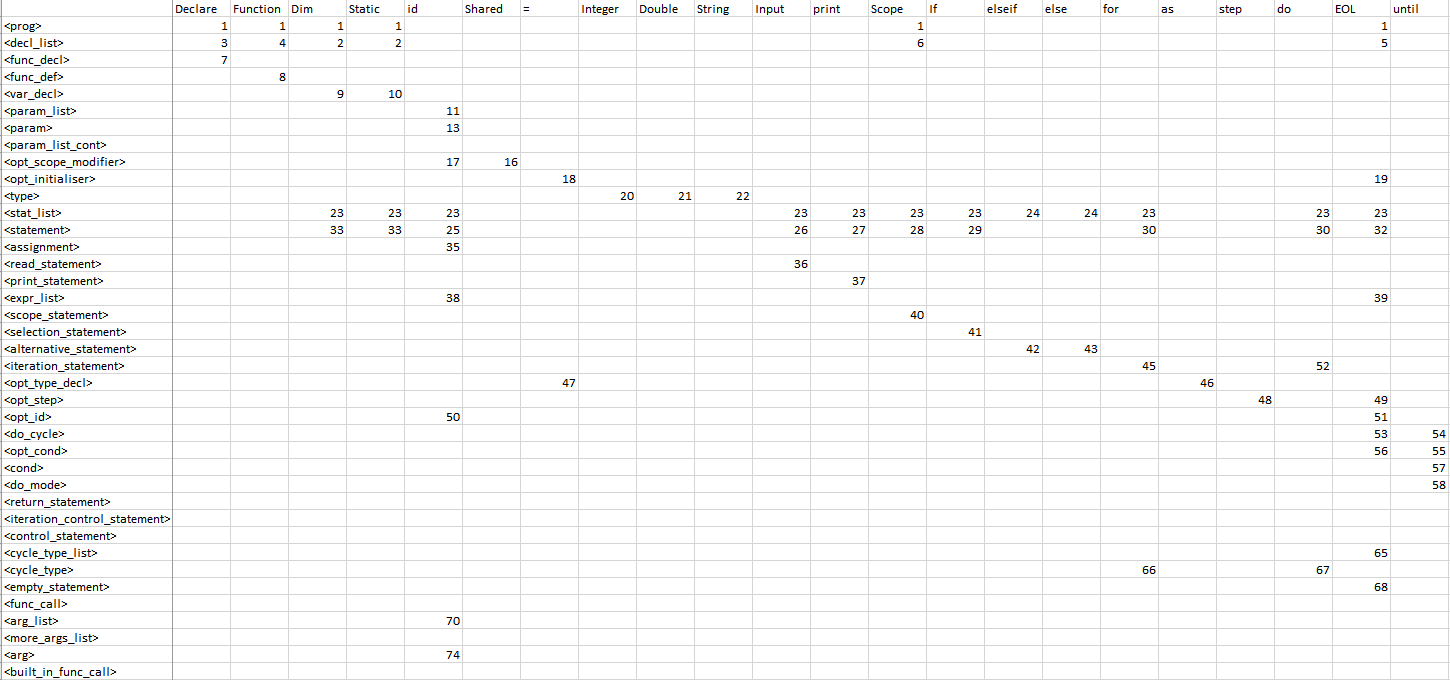
\includegraphics[width=\textwidth]{./attachments/ll_p1.png}

\hspace{2cm}

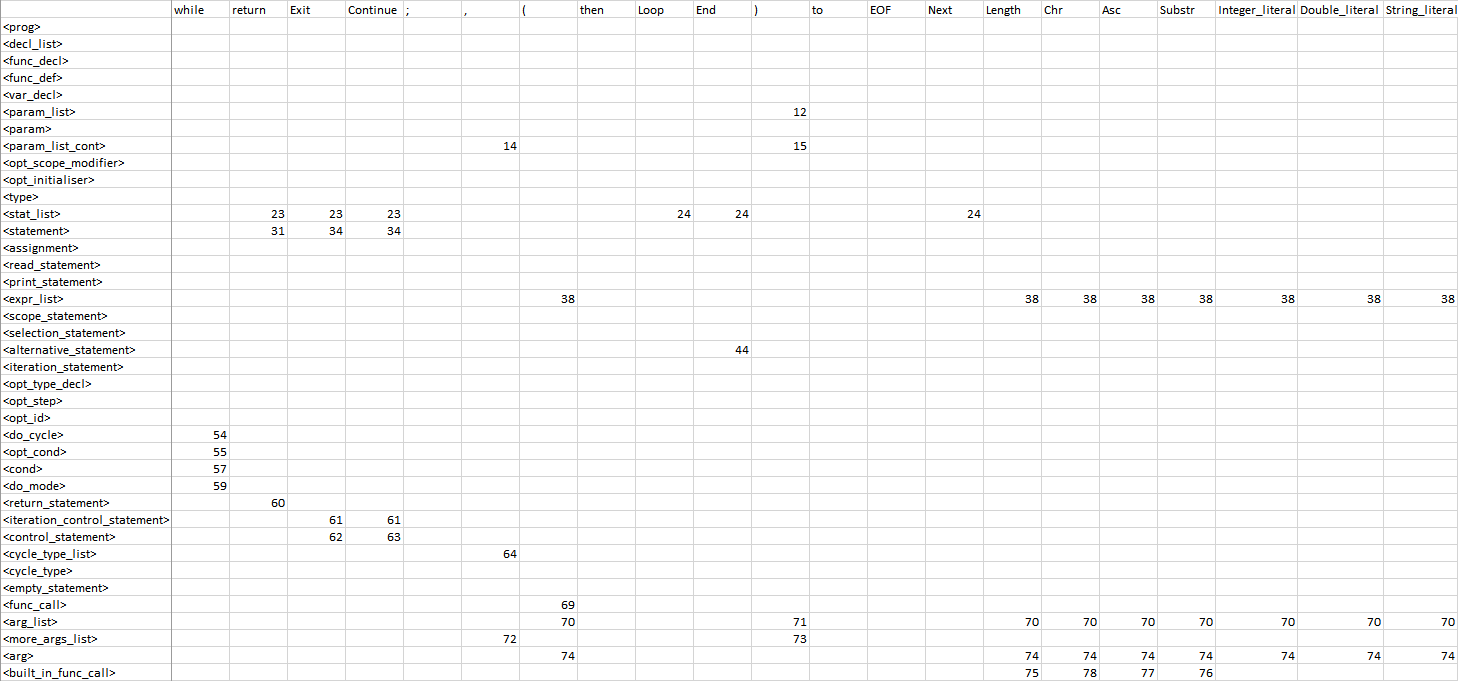
\includegraphics[width=\textwidth]{./attachments/ll_p2.png}

% Section: Appendix: Precedence table
\newpage
\label{fig::prec_table}
{\LARGE Figure 4: Precedence-table}
\fakesubsection{Precedence table}

\begin{table}[H]
\resizebox{\columnwidth}{!}{
\begin{tabular}[l]{| c | c | c | c | c | c | c | c | c | c | c | c | c | c | c | c | c | c | c |}
\hline
Top/Input & + & - & * & / & \textbackslash & = & < > & < & <= & > & >= & id & int\_lit & double\_lit & string\_lit & ( & ) & end \\ \hline
+ &	> &	> &	< &	< &	< &	> &	> &	> &	> &	> &	> &	< &	< &	< &	< &	< &	> &	> \\ \hline
- &	> &	> &	< &	< &	< &	> &	> &	> &	> &	> &	> &	< &	< &	< &	< &	< &	> &	> \\ \hline
* &	> &	> &	> &	> &	> &	> &	> &	> &	> &	> &	> &	< &	< &	< &	< &	< &	> &	> \\ \hline
/ &	> &	> &	> &	> &	> &	> &	> &	> &	> &	> &	> &	< &	< &	< &	< &	< &	> &	> \\ \hline
\textbackslash &	> &	> &	< &	< &	> &	> &	> &	> &	> &	> &	> &	< &	< &	< &	< &	< &	> &	> \\ \hline
= &	< &	< &	< &	< &	< &	   &     &	   &	    &    &    &	< &	< &	< &	< &	< &	> &	>  \\ \hline
< > &< & < & < & < & < &  &    &    &     &	    &    &	< &	< &	< &	< &	< &	> &	> \\ \hline
< &	< &	< &	< &	< &	< &	   &	    &    &    &     &   & < &	< &	< &	< &	< &	> &	> \\ \hline
<= & < & < & < & < & < & &    &    &     &     &   &	< & < &	< &	< &	< &	> &	> \\ \hline
> &	< &	< &	< &	< &	< &    &     &   &     &     &   &	< &	< &	< &	< &	< &	> &	> \\ \hline
>= & < & < & < & < & < & &    &    &     &    &    & < & < &	< &	< &	< &	> &	> \\ \hline
id &	> &	> &	> &	> &	> &	> &	> &	> &	> &	> &	> &    &     &    &    &    &	> &	> \\ \hline
int\_lit &	> &	> &	> &	> &	> &	> &	> &	> &	> &	> &	> & &    &    &    &    &	> & > \\ \hline
double\_lit &	> &	> &	> &	> &	> &	> &	> &	> &	> &	> &	> &  & &   &    &    & > &> \\ \hline
string\_lit  &  > &	> &	> &	> &	> &	> &	> &	> &	> &	> &	> &	  & &  &    &    & > &	> \\ \hline
( &	< &	< &	< &	< &	< &	< &	< &	< &	< &	< &	< &	< &	< &	< &	< &	< &	= &    \\ \hline	
) &	> &	> &	> &	> &	> &	> &	> &	> &	> &	> &	> &    &    &     &	    &    & > & > \\ \hline
end & < & < & < & < & < & < & < & < & < & < & < & < &	< &	< &	< &	< & end & \\ \hline	
\end{tabular}}
\end{table}

% Section: Appendix: Semantic stack rules
\newpage
\label{fig:sem_stack_rules}
{\LARGE Figure 4: Semantic stack rules}
\fakesubsection{Semantic stack rules}

\begin{enumerate}
\item \textbf{\textit{<prog>}} \\
Input: \hspace{3.288mm} - \\
Output: \enspace -

\item	\textbf{\textit{<decl\_list>}} \\
Input: \hspace{3.288mm} - \\
Output: \enspace -

\item \textbf{\textit{<var\_decl>}} \\
Input: \hspace{3.288mm} - \\
Output: \enspace -

\item \textbf{\textit{<opt\_initialiser>}} \\
Input: \hspace{3.288mm} - \\
Output: \enspace Expression with type (NO\_INIT in type if no initialiser)

\item \textbf{\textit{<type>}} \\
Input: \hspace{3.288mm} - \\
Output: \enspace Read type (Integer, Double or String)

\item \textbf{\textit{<opt\_scope\_modifier>}} \\
Input: \hspace{3.288mm} - \\
Output: \enspace Read scope modifier or NO\_MODIFIER

\item \textbf{\textit{<expr>}} \\
Input: \hspace{3.288mm} - \\
Output: \enspace Final expression resulting from the PSA algorithm

\item \textbf{\textit{<func\_decl>}} \\
Input: \hspace{3.288mm} - \\
Output: \enspace - 

\item \textbf{\textit{<func\_def>}} \\
Input: \hspace{3.288mm} - \\
Output: \enspace - 

\item \textbf{\textit{<param\_list>}} \\
Input: \hspace{3.288mm} - \\
Output: \enspace Number of parameters, followed by a reversed list of parameters

\item \textbf{\textit{<param>}} \\
Input: \hspace{3.288mm} - \\
Output: \enspace Type and name of the read parameter

\item \textbf{\textit{<param\_list\_cont>}} \\
Input: \hspace{3.288mm} Number of already read parameters \\
Output: \enspace Number of parameters, followed by a reversed list of parameters

\item \textbf{\textit{<cycle\_stat\_list>}} \\
Input: \hspace{3.288mm} List of cycle types with the caller on top (All only in non-recursive calls) \\
Output: \enspace Input

\item \textbf{\textit{<stat\_list>}} \\
Input: \hspace{3.288mm} List of cycle types with the caller on top (All only in non-recursive calls) \\
Output: \enspace Input

\item \textbf{\textit{<statement>}} \\
Input: \hspace{3.288mm} List of cycle types \\
Output: \enspace Input

\item \textbf{\textit{<iteration\_control\_statement>}} \\
Input: \hspace{3.288mm} List of cycle types \\
Output: \enspace Input

\item \textbf{\textit{<assigment>}} \\
Input: \hspace{3.288mm} - \\
Output: \enspace -

\item \textbf{\textit{<read\_statement>}} \\
Input: \hspace{3.288mm} - \\
Output: \enspace -

\item \textbf{\textit{<print\_statement>}} \\
Input: \hspace{3.288mm} - \\
Output: \enspace -

\item \textbf{\textit{<expr\_list>}} \\
Input: \hspace{3.288mm} Number of read expressions so far \\
Output: \enspace Number of read expressions, followed by a reversed list of these expressions

\item \textbf{\textit{<selection\_statement>}} \\
Input: \hspace{3.288mm} List of cycle types \\
Output: \enspace Input

\item \textbf{\textit{<iteration\_statement>}} \\
Input: \hspace{3.288mm} List of cycle types \\
Output: \enspace Input

\item \textbf{\textit{<empty\_statement>}} \\
Input: \hspace{3.288mm} - \\
Output: \enspace -

\item \textbf{\textit{<return\_statement>}} \\
Input: \hspace{3.288mm} - \\
Output: \enspace -

\item \textbf{\textit{<alternative\_statement>}} \\
Input: \hspace{3.288mm} List of cycle types (Only in non-recursive calls) \\
Output: \enspace Input

\item \textbf{\textit{<opt\_type\_decl>}} \\
Input: \hspace{3.288mm} - \\
Output: \enspace Read type or NO\_DECL

\item \textbf{\textit{<opt\_step>}} \\
Input: \hspace{3.288mm} - \\
Output: \enspace Step expression

\item \textbf{\textit{<opt\_id>}} \\
Input: \hspace{3.288mm} - \\
Output: \enspace Read identifier or NO\_ID

\item \textbf{\textit{<do\_cycle>}} \\
Input: \hspace{3.288mm} List of cycle types \\
Output: \enspace Input

\item \textbf{\textit{<opt\_cond>}} \\
Input: \hspace{3.288mm} - \\
Output: \enspace Condition expression and do mode,  or NO\_COND

\item \textbf{\textit{<cond>}} \\
Input: \hspace{3.288mm} - \\
Output: \enspace Condition expression, do mode

\item \textbf{\textit{<do\_mode>}} \\
Input: \hspace{3.288mm} - \\
Output: \enspace Do mode (Until or While)

\item \textbf{\textit{<control\_statement>}} \\
Input: \hspace{3.288mm} - \\
Output: \enspace Control statement (Continue or Exit)

\item \textbf{\textit{<cycle\_type\_list>}} \\
Input: \hspace{3.288mm} Initial cycle  \\
Output: \enspace Cycle type with number of occurences

\item \textbf{\textit{<cycle\_type>}} \\
Input: \hspace{3.288mm} -  \\
Output: \enspace Cycle type (For or Do)

\item \textbf{\textit{<built\_in\_func\_call>}} \\
Input: \hspace{3.288mm} -  \\
Output: \enspace Result expression containing the return value of the function call

\item \textbf{\textit{<func\_call>}} \\
Input: \hspace{3.288mm} -  \\
Output: \enspace Number of parameters, followed by a reversed list of expressions representing them

\item \textbf{\textit{<arg\_list>}} \\
Input: \hspace{3.288mm} -  \\
Output: \enspace Number of parameters, followed by a reversed list of expressions representing them

\item \textbf{\textit{<more\_args\_list>}} \\
Input: \hspace{3.288mm} Number of already read parameters followed by a reversed list of expressions representing them  \\
Output: \enspace Number of parameters, followed by a reversed list of expressions representing them

\item \textbf{\textit{<arg>}} \\
Input: \hspace{3.288mm} -  \\
Output: \enspace Read argument expression
\end{enumerate}

%%%%%%%%%%		End of the Document 				%%%%%%%%%%
\end{document}